%
% intro.tex
%


Computer games are growing in importance at an astonishing speed. Games have since long catched up with Hollywood in economic terms \cite{3}, their use base for entertainment purposes is huge \cite{MILLIONS_USERS} and even more importantly games are more and more being studied as the next frontier in engaging education \cite{FUN_IO,GAMES_FIRST_APPROACH}.

Up until not many years ago, computer graphics were the main source of innovation in games. As realtime computer graphics is approaching an exceptionally high mark some focus is shifting away from making better looking games and is instead focusing on \textit{the interactive experience}. An example of this phenomenon is the fact that the current generation of consoles has moved away from the traditional 4-year update cycle and instead has experimented with novel forms of user interaction \cite{KINECT}.

The papers we discuss \cite{SGL1,SGL2,SGL3,SGL4} support this view, and add that a very important aspect of the interactive experience is the AI (artificial intelligence) of the animated characters that play the part of the various actors of the game. Traditionally, games have improved game AI along two axes:

\begin{itemize}
\item character depth;
\item number of characters.
\end{itemize}

Character depth has been used in order to build fewer characters that interact with the user for a long duration. These characters must be believable, and so they must behave smartly and sometimes even convey strong emotions: the story villain and the player's small party of followers must all be engaging and credible. To this end, expert systems have been employed to various degrees in games \cite{14,12,17}.

Deep characters are very computationally expensive. Modern AI techniques would be unfeasible if applied to more than a handful of such characters. Strategy games and massively multiplayer online role playing games (and open world games in general) require AI techniques that are capable of supporting hundreds or thousands of animated characters \cite{2,23}. In these games character behaviors are often governed by simple state machines. The combination of many such simple AIs makes for interesting emergent behaviors that combine into a compelling gameplay. A risk that is ever-present is that of dumbing down the AI intelligence in order to fit the required number of units. 

\begin{figure*}
\begin{center}
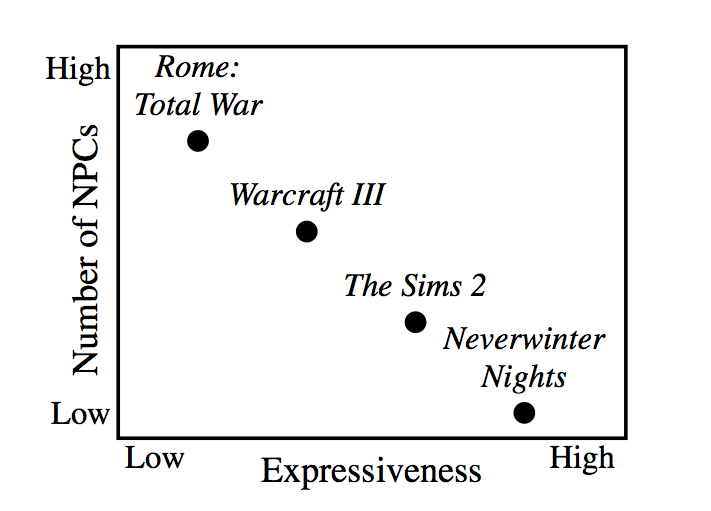
\includegraphics[scale=0.3]{characters_ai.png}
\end{center}
\label{fig:characters_ai}
\caption{AI complexity versus number of characters}
\end{figure*}

The above distinction about in-game AI is summarized in Figure 1.

AI in games in practice is often data-driven. Some scripting system is attached to the game engine in order to allow customization of AI behaviors. In their simplest form scripts are simply a (possibly very large) set of configuration parameters that customize the fixed units behavior. More advanced scripting systems \cite{18,24} allow coding detailed aspects of the characters behaviors in fully-fledged programming languages.

The authors goal is to create a data-driven AI system that is capable of expressing any point in the ``scripting space'' described above, that is they wish to be able to express scripts that are both complex to animate believable and smart characters and capable of doing so efficiently for hundreds or thousands of characters.
